% \input{\pLocalSlides "slide-Models-Radar-Cross-Sections-for-Satellites"}

\begin{frame}{Models of Radar Cross Sections for Satellites}
    \centering
    \begin{columns}[c,onlytextwidth]
        % Left Column: Satellite Image
        \begin{column}{0.4\textwidth}
            \centering
            \begin{tikzpicture}
                \node[inner sep=0pt] at (0,0) 
                {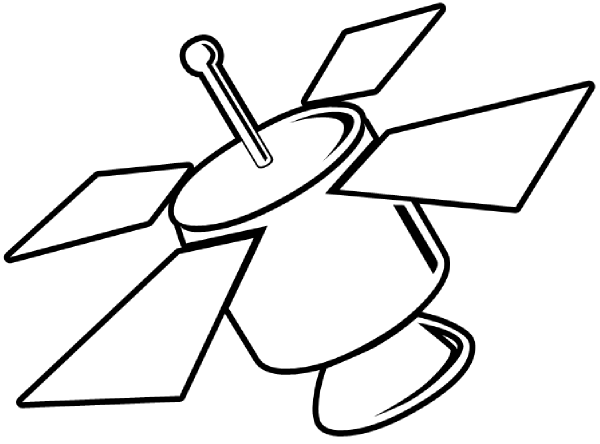
\includegraphics[width=0.9\linewidth]{\pLocalGraphics/satellites/satellite-outline-hi.png}};
            \end{tikzpicture}
        \end{column}

        % Right Column: Spherical Harmonics Expansion
        \begin{column}{0.6\textwidth}
            \centering
            \textbf{\large Spherical Harmonics Expansion} \\[0.8em]
            \begin{align*}
                f(\theta, \phi) \approx & \; \textcolor{blue}{a_{0,0}} R_{0}^{0}(r)Y_0^0 
                + \textcolor{blue}{a_{1,-1}} Y_1^{-1} \\
                & + \textcolor{blue}{a_{1,0}} Y_1^0 
                + \textcolor{blue}{a_{1,1}} Y_1^1 
                + \dots
            \end{align*}
        \end{column}
    \end{columns}

    % Bottom Line: Y_n^m Definition Spanning the Slide
    \vspace{1em}
    \textbf{where}
    \[
    Y_n^m(\theta, \phi) = 
    \sqrt{\frac{(2n + 1)(n - m)!}{4\pi (n + m)!}} P_n^m(\cos \theta) e^{im\phi}
    \]
\end{frame}

\endinput  %  ==  ==  ==  ==  ==  ==  ==  ==  ==
